\chapter{Grafteori}
Følgende kapitel er skrevet med afsæt i \citep{dmat}.

Grafer er diskrete strukturer, som bruges til at modellere relationer mellem forskellige objekter.  Graferne varierer alt efter deres type og funktion, og har mange forskellige egenskaber. De mange forskellige egenskaber betyder, at problemer i næsten enhver tænkelig disciplin kan løses ved hjælp af grafmodeller. Vi vil eksempelvis i dette projekt benytte grafteori og princippet om den længste vej til at optimere et gaslager. En graf er givet ved:
\begin{defn}[Graf]
En \emph{graf}, $G = (V,E)$, består af $V$, som er en mængde \emph{knuder} hvor $V \neq \emptyset$ og en mængde \emph{kanter}, $E$, som er \emph{incident} med disse knuder. 
\end{defn}

Vi siger en tilfældig kant, $e \in E$, er incident med knuderne $u$ og $v$, hvis kanten har $u$ og $v$ som dens endeknuder, hvor $u, v \in V$. Her siger man også at $u$ og $v$ er \emph{naboer}. Hvis en kant kun er incident med én knude, er der tale om en \emph{løkke}.
Det fremgår af definitionen, at en graf ikke kan have nul knuder, men en lignende afgrænsning i den anden ende eksisterer ikke. Der kan dermed være uendeligt mange knuder. På samme måde gælder det for kanter, at der kan være mellem nul og uendeligt. Hvis mindst et af disse tilfælde gør sig gældende, kaldes det en \emph{uendelig graf}. Ellers kaldes det en \emph{endelig graf}, og det er denne type, som vi beskæftiger os med i projektet.
Knuderne illustreres ofte som prikker, mens kanterne repræsenteres af streger eller pile, der forbinder disse prikker. 

\section{Graftyper}
En graf er, som tidligere nævnt, en struktur med knuder og kanter. Den er givet ved definitionen:
\begin{defn}
[Simpel graf] 
En graf, $G=(V,E)$, består af $V$, en mængde af \emph{knuder}, hvor $V = \emptyset$, og en mængde af \emph{kanter}, $E \subseteq \{\{u,v\}|u,v \in V\}$.
\end{defn}
Det fremgår af definitionen, at en graf ikke kan have nul knuder, men en lignende afgrænsning i den anden ende eksisterer ikke. Der kan dermed være uendeligt mange knuder. På samme måde gælder det for kanter, at der kan være mellem nul og uendeligt. Hvis mindst et af disse tilfælde gør sig gældende, kaldes det en \emph{uendelig graf}. Ellers kaldes det en \emph{endelig graf}, og det er denne type, som vi beskæftiger os med i projektet.
Ydermere, ses det i definitionen, at hver kant forbinder én eller to knuder. For en simpel graf gælder det, at ingen kanter forbinder et punkt med sig selv. Der må altså ikke være løkker. 

\begin{figure}[H]
\centering
	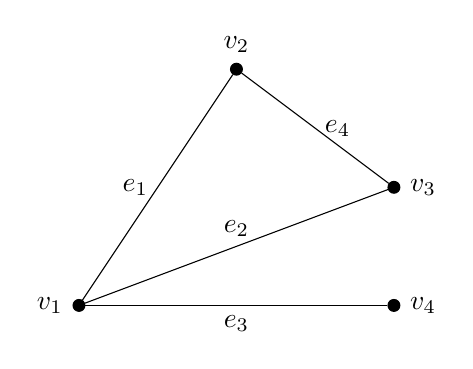
\begin{tikzpicture}

      \tikzset{enclosed/.style={draw, circle, inner sep=0pt, minimum size=.15cm, fill=black}}
%% Vertices
      	\node[enclosed, label={left: $v_1$}] (v1) at (0,0) {};
      	\node[enclosed, label={above: $v_2$}] (v2) at (2,3) {};
    	\node[enclosed, label={right: $v_3$}] (v3) at (4,1.5) {};
  	    \node[enclosed, label={right: $v_4$}] (v4) at (4,0) {};
%Edges
		\path (v1) edge node[midway, left] {$e_1$} (v2);
		\path (v1) edge node[midway, above] {$e_2$} (v3);
		\path (v1) edge node[midway, below] {$e_3$} (v4);
		\path (v2) edge node[midway, right] {$e_4$} (v3);

	\end{tikzpicture}
	\caption{En simpel graf}
	\label{fig.simpel}
\end{figure}



I kontrast til den simple graf finder vi multigrafen. For denne type graf skal der være flere kanter, der forbinder det samme knudepar. Der må stadig ikke optræde løkker.

\begin{figure}[H]
\centering
	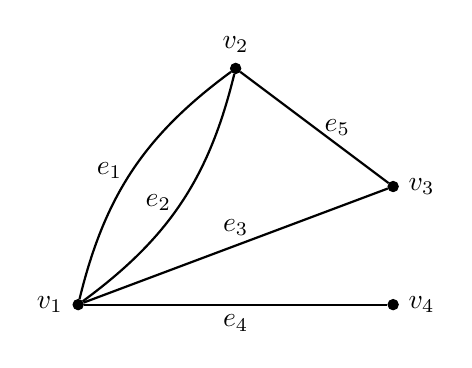
\begin{tikzpicture}

      \tikzset{enclosed/.style={draw, circle, inner sep=0pt, minimum size=.13cm, fill=black}}
%% Vertices
      	\node[enclosed, label={left: $v_1$}] (v1) at (0,0) {};
      	\node[enclosed, label={above: $v_2$}] (v2) at (2,3) {};
    	\node[enclosed, label={right: $v_3$}] (v3) at (4,1.5) {};
  	    \node[enclosed, label={right: $v_4$}] (v4) at (4,0) {};
%Edges
		\path[thick] (v1) edge [bend right=20] node[midway, left] {$e_2$} (v2);
		\path[thick] (v2) edge [bend right=20] node[midway, left] {$e_1$} (v1);
		\path[thick] (v1) edge node[midway, above] {$e_3$} (v3);
		\path[thick] (v1) edge node[midway, below] {$e_4$} (v4);
		\path[thick] (v2) edge node[midway, right] {$e_5$} (v3);

	\end{tikzpicture}
	\caption{En multigraf.}
	\label{fig.multi}
\end{figure}


En pseudograf er en graf, der \emph{kan} indeholde løkker, men generelt set er alle grafer pseudografer. Man vil dog kun bruge betegnelsen, pseudograf, hvis den indeholder en løkke, da det ellers vil være mere præcist at kalde den en simpel eller multigraf. Vi ser i eksemplet herunder, at der er to kanter, der forbinder $v_{1}$ og $v_{2}$, og der er en løkke ved $v_{4}$.

\begin{figure}[H]
\centering
	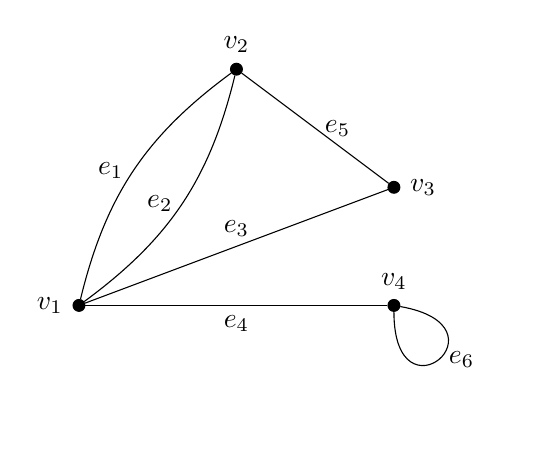
\begin{tikzpicture}[every loop/.style={}]
      \tikzset{enclosed/.style={draw, circle, inner sep=0pt, minimum size=.15cm, fill=black}}
%% Vertices
      	\node[enclosed, label={left: $v_1$}] (v1) at (0,0) {};
      	\node[enclosed, label={above: $v_2$}] (v2) at (2,3) {};
    	\node[enclosed, label={right: $v_3$}] (v3) at (4,1.5) {};
  	    \node[enclosed, label={above: $v_4$}] (v4) at (4,0) {};
%Edges
		\path (v1) edge [bend right=20] node[midway, left] {$e_2$} (v2);
		\path (v2) edge [bend right=20] node[midway, left] {$e_1$} (v1);
		\path (v1) edge node[midway, above] {$e_3$} (v3);
		\path (v1) edge node[midway, below] {$e_4$} (v4);
		\path (v2) edge node[midway, right] {$e_5$} (v3);
		\path (v4) edge [out=270,in=350,looseness=35] node[right] {$e_6$} (v4);
	\end{tikzpicture}
	\caption{En pseudograf med en løkke.}
	\label{fig.pseudo}
\end{figure}



\subsection{Orienterede grafer og ikke-orienterede grafer}
En anden typisk grafopdeling er opdelingen i orienterede og ikke-orienterede grafer. De grafer, vi har kigget på indtil videre, er ikke-orienterede grafer. For en orienteret graf gælder det, at grafens kanter er retningsbestemte. Dette er ofte illustreret med pile. Den har dermed en startknude og en endeknude. Disse grafer er defineret ved:

\begin{defn}
[Orienteret graf] 

En orienteret graf, $G=(V,E)$, består af $V$, en m�ngde knuder, hvor $V \neq \emptyset$, og en mængde orienterede kanter, $E$. Hver orienterede kant forbinder et par knuder, $(u,v)$, hvor startknuden, $u$, er tilstødende til endeknuden, $v$. 


\input{fig/tikz/grafer/graftyper/orienteretgraf}

Der kan foruden disse to også være tale om blandede grafer, som er grafer med både orienterede og ikke-orienterede kanter. Orienterede grafer kan ligesom ikke-orienterede grafer indeholde løkker og flere ensrettede kanter, der forbinder det samme par knuder, men hvis dette ikke er tilfældet, kaldes det en orienteret simpel graf. En orienteret simpel graf må også indeholde to modsatrettede kanter mellem det samme knudepar. Dermed kan en kant gå fra $v$ til $u$, selvom en anden kant går fra $u$ til $v$. Hvis der derimod optræder løkker eller flere ensrettede kanter mellem et eller flere knudepar, kaldes det en orienteret multigraf.  

Egenskaberne for de forskellige grafer kan ses herunder:


\begin{center}
\begin{tabular}{ |p{4cm}|p{3cm}|p{3cm}|p{2cm}|  }
 \hline
 \multicolumn{4}{|c|}{Grafer} \\
 \hline
 Type & Kanter & Flere kanter per knudepar tilladt & Løkker tilladt\\
 \hline
 Simpel graf   & Ikke-orienterede    & Nej &   Nej\\
 Multigraf &   Ikke-orienterede & Ja   & Nej\\
 Pseudograf & Ikke-orienterede & Ja &  Ja\\
 Simpel orienteret graf    & Orienterede & Nej &  Nej\\
 Orienteret multigraf &  Orienterede  & Ja & Ja\\
 Blandet graf & Ikke-orienterede og orienterede  & Ja   & Ja\\
 \hline
\end{tabular}
\end{center}

Fordi kanterne i grafer med orienterede kanter er ordnede par, kan definitionen af knudens grader være antallet af kanter, der har denne knude som begyndelsesknude, eller antallet af kanter, der har denne knude som endeknude:
\begin{defn}
[Graden af en orienteret graf] 
I en graf med orienterede kanter er ind-graden, betegnet ved $deg^{-}(v)$, antallet af kanter med $v$ som deres endeknude. Ud-graden, betegnet ved $deg^{+}(v)$, er antallet af kanter med $v$ som deres startknude.
\end{defn}
Vi vil i projektet beskæftige os med orienterede grafer, da det er denne type, vi bruger til optimering af gaslageret. I vores tilfælde vil vi tildele vores orienterede kanter vægt, hvilket beskrives senere i projektet.


\section{Repræsentation af grafer}
Inden for grafteori er der forskellige måder at repræsentere en graf på. Normalvis repræsenterer man en graf med punkter og streger og/eller pile, men de kan også repræsenteres ved brug af lister og matricer. Disse metoder giver et mere praktisk overblik over grafer.

\subsection{Nabolister}
En måde at repræsentere en graf på er ved at lave en naboliste. Nabolister er tabeller, der giver en oversigt over hvilke knuder, der er forbundet med andre knuder. Dog vil man ikke kunne se, hvis der er parallelle kanter. En naboliste er bygget op således, at knuden, man vil beskrive, er i venstre side af tabellen, og naboknuderne er skrevet i højre side. \\

%\begin{figure}[h]
%  \centering
%  \begin{tikzpicture}
%    \node[point] at (1,2) ($v_{2}$) [label=above:\(A\)] {};
%    \node[point] at (3,2) ($v_{4}$) [label=above:\(B\)] {};
%    \node[point] at (4,1) ($v_{7}$) [label=right:\(C\)] {};
%    \node[point] at (2,0) ($v_{5}$) [label=below:\(D\)] {};
%    \node[point] at (3,0) ($v_{6}$) [label=below:\(E\)] {};
%    \node[point] at (1,1) ($v_{3}$) [label=left:\(F\)] {};
%    \node[point] at (0,2) ($v_{1}$) [label=below:\(G\)] {};
%
%    \footnotesize
%    \draw ($v_{2}$) -- ($v_{1}$);
%    \path ($v_{3}$) edge [bend left] ($v_{4}$);
%    \draw ($v_{2}$) -- ($v_{3}$);
%    \path ($v_{3}$) edge [bend right] ($v_{4}$);
%    \draw ($v_{4}$) -- ($v_{5}$);
%    \draw ($v_{4}$) -- ($v_{6}$);
%    \draw ($v_{4}$) -- ($v_{5}$);
%    \draw ($v_{7}$) -- ($v_{6}$);
%    \draw ($v_{7}$) to [out=315,in=45,looseness=50] ($v_{7}$);
%    \draw ($v_{6}$) -- ($v_{5}$);
%    \draw ($v_{5}$) -- ($v_{3}$);
%    \draw ($v_{3}$) -- ($v_{1}$);
%  \end{tikzpicture}
%  \caption{Ikke-orienteret pseudograf.}
%  \label{fig:ikke-orienteret-pseudo}
%\end{figure}

\begin{center}
	\begin{tabular}{ |p{4cm}||p{3cm}|}
	 	\hline
 		\multicolumn{2}{|c|}{Naboliste til figur \ref{fig:ikke-orienteret-pseudo}} \\
 		\hline
 		Knuder & Naboknuder\\
 		\hline
 		A & F,G \\
		B & C,D,E,F \\
		C & B,E,C \\
		D & B,E,F \\
		E & B,C,D \\
		F & A,B,D,G \\
		G & A,F \\
 	\hline
 	\label{tab:naboliste} 	
	\end{tabular}
	%\caption{Naboliste til figur \ref{fig:ikke-orienteret-pseudo}
\end{center}
Ud fra tabellen ses, at knuden B har naboknuderne C, D, E og F, men man kan ikke se, at der er en ekstra kant mellem B og F. Dog kan man se, at C har en løkke, da den er nabo til sig selv.

\begin{figure}[H]
  \centering
  \begin{tikzpicture}
    \node[point] at (1,2) (A) [label=above:\(A\)] {};
    \node[point] at (3,2) (B) [label=above:\(B\)] {};
    \node[point] at (4,1) (C) [label=right:\(C\)] {};
    \node[point] at (2,0) (D) [label=below:\(D\)] {};
    \node[point] at (3,0) (E) [label=below:\(E\)] {};
    \node[point] at (1,1) (F) [label=left:\(F\)] {};
    \node[point] at (0,2) (G) [label=below:\(G\)] {};

    \footnotesize
    \path [->] (A) edge [bend left] (G);
    \path [->] (A) edge [bend right] (G); 
    \path [->] (F) edge [bend left] (B);
    \draw [<-](A) -- (F);
    \path [<-](F) edge [bend right] (B);
    \draw [->](B) -- (D);
    \draw [<-](B) -- (E);
    \draw [<-](B) -- (C);
    \draw [->](C) -- (E);
    \draw [->](C) to [out=315,in=45,looseness=50] (C);
    \draw [<-](E) -- (D);
    \draw [->](D) -- (F);
    \draw [->](F) -- (G);
  \end{tikzpicture}
  \caption{Orienteret pseudograf.}
  \label{fig:orienteret-pseudo}
\end{figure}

%\begin{center}
%	\begin{tabular}{ |p{4cm}||p{3cm}|}
%	 	\hline
% 		\multicolumn{2}{|c|}{Naboliste til figur \ref{fig:orienteret-pseudo} \\
% 		\hline
% 		Knuder & Naboknuder\\
% 		\hline
% 		A & G \\
%		B & D,F \\
%		C & B,E,C \\
%		D & E,F \\
%		E & B \\
%		F & A,B,G \\
%		G &  \\
% 	\hline
% 	\label{tab:naboliste1}
%	\end{tabular}
%\end{center}

\ref{tab:naboliste1} viser en oversigt over den orienterede grafs (Figur \ref{fig:orienteret-pseudo}) naboknuder. Kigger man på B og F i tabellen, kan man se, at der er parallelle kanter, da kanterne er orienteret i hver deres retning. Kigger man på A og G, kan man ikke se, at der er parallelle kanter mellem A og G, da begge kanter er orienteret fra A til G.

\subsection{Nabomatricer}
En anden mulighed for at repræsentere en graf er ved brug af \emph{nabomatricer}. Nabomatricer er bedre, når grafen har mange kanter, da man her kan se hvor mange kanter et givent knudepar har.
En nabomatrix kan beskrives som en $N=m \times m$-matrix, hvor $m$ er afhængig af knudemængden $V=\{v_1, v_2, \dotsc, v_m\}$. Hvis man har en simpel graf, $G=(V,E)$, vil matricen være en 0-1-matrix, da en simpel graf kun kan have en kant mellem to knuder. Når der er en kant mellem to  vilkårlig knuder, $a_{ij}=(v_i,v_j)$,  vil den få notationen 1, hvis der derimod ikke er en kant, får den notationen 0.
Det kan også skrives som
\begin{equation}
	a_{ij} =	
	\begin{cases}
		1 \mbox{ hvis } (v_i,v_j) \\
		0 \mbox{ ellers }.
	\end{cases}
\end{equation}

\begin{figure}[H]
  \centering
  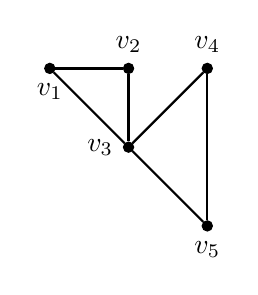
\begin{tikzpicture}
  \tikzset{enclosed/.style={draw, circle, inner sep=0pt, minimum size=.13cm, fill=black}}
  	\node[enclosed] at (0,2) (v1) [label=below:\(v_1\)] {};
    \node[enclosed] at (1,2) (v2) [label=above:\(v_2\)] {};
    \node[enclosed] at (1,1) (v3) [label=left:\(v_3\)] {};
    \node[enclosed] at (2,2) (v4) [label=above:\(v_4\)] {};
    \node[enclosed] at (2,0) (v5) [label=below:\(v_5\)] {};
    
	\path[thick] (v1) edge node {} (v2);
	\path[thick] (v1) edge node {} (v3);
	\path[thick] (v2) edge node {} (v3);
	\path[thick] (v4) edge node {} (v3);
	\path[thick] (v5) edge node {} (v3);   
	\path[thick] (v4) edge node {} (v5); 

  \end{tikzpicture}
  \caption{Ikke-orienteret, simpel graf til matrix.}
  \label{fig:stm}
\end{figure}

Nabomatricen nedenfor, viser en matrix over \autoref{fig:stm}.
\begin{equation}
	\begin{bmatrix}
		&v_1&v_2&v_3&v_4&v_5 \\
		v_1&0&1&1&0&0 \\
		v_2&1&0&1&0&0 \\
		v_3&1&1&0&1&1 \\
		v_4&0&0&1&0&1 \\
		v_5&0&0&1&1&0 \\
	\end{bmatrix}
\end{equation}

En matrix over en graf med flere parallelle kanter mellem to knuder vil se ud således. Matricen nedenfor viser en matrix over \autoref{fig:ikke-orienteret-pseudo}.

\begin{equation}
	\begin{bmatrix}
	&v_1&v_2&v_3&v_4&v_5&v_6&v_7& \\
	v_1&0&1&1&0&0&0&0 \\
	v_2&1&0&1&0&0&0&0 \\
	v_3&1&1&0&2&1&0&0 \\
	v_4&0&0&2&0&1&1&1 \\
	v_5&0&0&1&1&0&1&0 \\
	v_6&0&0&0&1&1&0&1 \\
	v_7&0&0&0&1&0&1&1 \\	
	\end{bmatrix}
\end{equation}

Det kan ses, at der er 2 kanter, der er incidente med knudeparret $v_3$ og $v_4$. Derudover kan det ses, at der er en løkke ved $v_7$.



\section{Veje}
Vi har indtil videre snakket om knuder, og hvordan de som knudersæt forbindes med kanter. I dette afsnit vil vi udvide det til at snakke om veje, som er sekvenser af disse kanter. Hvis der er tale om ikke-orienterede grafer, er veje defineret ved:
\begin{defn}
[Veje] 
Lad $n \in \N _0$  og $G$ være en ikke-orienteret graf. En vej af længde $n$, fra $u$ til $v$, i $G$ er en sekvens af $n$ kanter $e_{1},e_{2},\cdots,e_{n}$ for $G$, for hvilket der eksisterer en sekvens, $x_{0}=u$ og $x_{1},x_{2},\cdots,x_{n-1}$,$x_{n}=v$, af knuder sådan at $e_{i}$ har, for $i=1,2,\cdots,n$, endeknudererne $x_{i-1}$ og $x_{i}$. Når grafen er simpel, betegnes vejen ved dens knudesekvens $x_{o},x_{1},\cdots,x_{n}$. Vejen passeret igennem knuderne $x_{o},x_{1},\cdots,x_{n-1}$ eller krydse kanterne $e_{1},e_{2},\cdots,e_{n}$. En vej er simpel, hvis den ikke krydser den samme kant mere end én gang.
\end{defn}
Kigger vi derimod på veje med orienterede grafer, som er det vi beskæftiger os med i problemet, ser definitionen en smule anderledes ud:
\begin{defn}
[Veje] 
Lad $n \in \N _0$ og $G$ være en orienteret graf. En vej af længde $n$ fra $u$ til $v$ i $G$ er en sekvens af kanter $e_{1},e_{2},\cdots,e_{n}$ for $G$, sådan at $e_{1}$ er forbundet med $(x_{0},x_{1})$, $e_{2}$ er forbundet med $(x_{1},x_{2})$ og så videre frem til $e_{n}$, som er forbundet med $(x_{n-1},x_{n})$. Her er $x_{0}=u$ og $x_{n}=v$. Hvis alle knudesæt er forbundet med højst én kant per sæt, betegner vi denne  vej ved dets knudesekvens $x_{o},x_{1},\cdots,x_{n}$. En vej er simpel, hvis den ikke krydser den samme kant mere end én gang.
\end{defn}

\begin{figure}[H]
\centering
	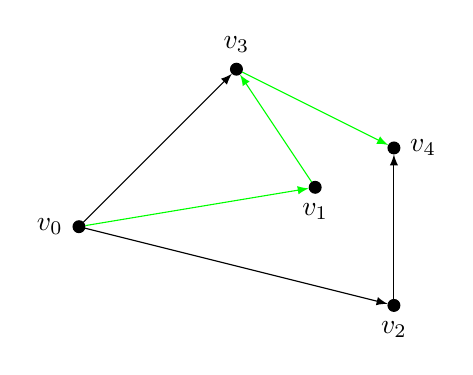
\begin{tikzpicture}

      \tikzset{enclosed/.style={draw, circle, inner sep=0pt, minimum size=.15cm, fill=black}}
%% Vertices
      	\node[enclosed, label={left: $v_0$}] (v0) at (0,2) {};
      	\node[enclosed, label={below: $v_1$}] (v1) at (3,2.5) {};
    		\node[enclosed, label={below: $v_2$}] (v2) at (4,1) {};
  	    \node[enclosed, label={above: $v_3$}] (v3) at (2,4) {};
     	\node[enclosed, label={right: $v_4$}] (v4) at (4,3) {};
%Edges
		\path [->, >=latex, green](v0) edge node[midway, sloped, above] {} (v1);
		\path [->, >=latex](v0) edge node[midway, sloped, above] {} (v2);
		\path [->, >=latex](v0) edge node[midway, above] {} (v3);
		\path [->, >=latex, green](v1) edge node[near end, sloped, below] {} (v3);
		\path [->, >=latex](v2) edge node[midway, below] {} (v4);
		\path [->, >=latex, green](v3) edge node[near end, sloped, above] {} (v4);

	\end{tikzpicture}
	\caption{Eksempel på en orienteret simpel graf og en vej fra $v_{0}$ til $v_{4}$}
	\label{fig.vaegtetopg}
\end{figure}


Antallet af veje mellem to knuder i grafen kan findes ved hjælp af nabomatricer, som vi diskuterede i forrige afsnit.
\begin{thm}
[Antallet af veje mellem to knuder] 
Lad G være en vilkårlig graf med nabomatricen
\textbf{$A$} med grafens knuder i rækkefølgen $v_{1},v_{2},\cdots,v_{n}$. Antallet af forskellige veje med længde $r$ fra $v_{i}$ til $v_{j}$ vil da være lig den $(i,j)$'te indgang af \textbf{$A^{r}$}.
\end{thm}

\begin{proof}
Bevis: Lad G være en graf med nabomatricen 
\textbf{$A$}, hvor vi antager, at knuderne i $G$ har rækkefølgen $v_{1},v_{2},\cdots,v_{n}$. Antallet af veje fra $v_{i}$ til $v_{j}$ af længde 1 er da den $(i,j)$'te indgang til 
\textbf{$A$}. Dette skyldes, at det blot er antallet af kanter fra $v_{i}$ til $v_{j}$.
Vi antager, at den $(i,j)$'te indgang til 
\textbf{${A^r}$} er antallet af forskellige veje, som går fra $v_{i}$ til $v_{j}$ og som har længden $r$. Dette er hypotesen, vi ønsker at bekræfte.
Vi ser på nabomatricen \textbf{$A^{r+1}$}. 
\textbf{$A^{r+1}$} er det samme som 
\textbf{$A^{r}$}$\cdot$\textbf{$A$}, og derfor er den $(i,j)$'te indgang af \textbf{$A^{r+1}$} lig med $b_{i1}a_{1j} + b_{i2}a_{2j} +\cdots+ b_{in}a_{nj}$. Her er $b_{ik}$  den $(i,k)$'te indgang til 
\textbf{$A^{r}$}, som ifølge vores hypotese er antallet af veje fra $v_{i}$ til $v_{k}$ med længde $r$.
En vej af længde $r + 1$ fra $v_{i}$ til $v_{k}$ er lavet ud fra en vej med længden $r$ fra begyndelsesknuden $v_{i}$ og hen til en mellemliggende knude $v_{k}$ samt den kant, der går fra $v_{k}$ til $v_{j}$. Vi ved fra kombinatorik, at antallet af muligheder er lig produktet af mulighederne ved første udfald og mulighederne ved andet udfald. Vi betegner antallet af veje med længden $r$ fra $v_{i}$ til $v_{k}$ med $b_{ik}$ og antallet af kanter fra $v_{k}$ til $v_{j}$ med $a_{kj}$ Finder vi produktet af dette for alle mellemliggende knuder, $v_{k}$, fås det ønskede resultat.
\end{proof}

\begin{exmp}
Vi starter med at kigge på en graf og den tilhørende nabomatrice:
\begin{figure}[H]
\centering
	\begin{tikzpicture}

      \tikzset{enclosed/.style={draw, circle, inner sep=0pt, minimum size=.15cm, fill=black}}
%% Vertices
      	\node[enclosed, label={left: $v_0$}] (v0) at (1,2) {};
      	\node[enclosed, label={above: $v_1$}] (v1) at (3,4) {};
    	\node[enclosed, label={below: $v_2$}] (v2) at (1,0) {};
  	    \node[enclosed, label={right: $v_3$}] (v3) at (5,2) {};
     	\node[enclosed, label={below: $v_4$}] (v4) at (5,0) {};
%Edges
		\path (v0) edge node[midway, sloped, above] {} (v1);
		\path (v0) edge node[midway, sloped, above] {} (v2);
		\path (v0) edge node[midway, above] {} (v3);
		\path (v1) edge node[near end, sloped, below] {} (v3);
		\path (v2) edge node[midway, below] {} (v4);
		\path (v3) edge node[near end, sloped, above] {} (v4);

	\end{tikzpicture}
	\caption{Eksempel på en ikke-orienteret simpel graf}
	\label{fig.vaegtetopg}
\end{figure}


\begin{equation}
A=\begin{bmatrix}
    0&1&1&1&0\\
    1&0&0&1&0\\
    1&0&0&0&1\\
    1&1&0&0&1\\
    0&0&1&1&0\\
\end{bmatrix}
\end{equation}


Vi ønsker at finde ud af hvor mange veje med en længde på 4, der går fra $v_0$ til $v_4$. Det ses i nabomatricen, at $v_0$ har 3 naboer, nemlig $v_1$, $v_2$ og $v_3$. Fortsætter vi, kan vi se, at $v_1$ har $v_0$ og $v_3$ som naboer, $v_2$ har $v_0$ og $v_4$, og $v_3$ har $v_0$, $v_1$ og $v_4$ som naboer. Fortsætter vi, så vi finder alle tænkelige veje med længder på 3, får vi, at der er 18 forskellige veje, der alle starter i $v_0$ og har en længde på 4. Vi skal nu finde de veje der ved at tilføje en kant ender i $v_4$. Vi kan se, at $v_4$ har $v_2$ og $v_3$ som naboer. Vi finder derfor de veje der starter i $v_0$ og slutter i $v_2$ med længden 3 og derefter dem der slutter i $v_3$ med længden 3. På denne måde udnytter vi, hvad vi skrev i beviset, nemlig at
\textbf{$A^{r+1}$} er lig med $b_{i1}a_{1j} + b_{i2}a_{2j} +\cdots+ b_{in}a_{nj}$
Her er $b_{ik}$ antallet af veje fra $v_{i}$ til ${v_k}$. I vores eksempel er $v_{i}=v_{0}$, ${v_k}=v_{2}$ og ${v_k}=v_{3}$ og \textbf{$A^{r+1}$}=\textbf{$A^{3+1}$}. 
 
\begin{figure}[H]
\centering
	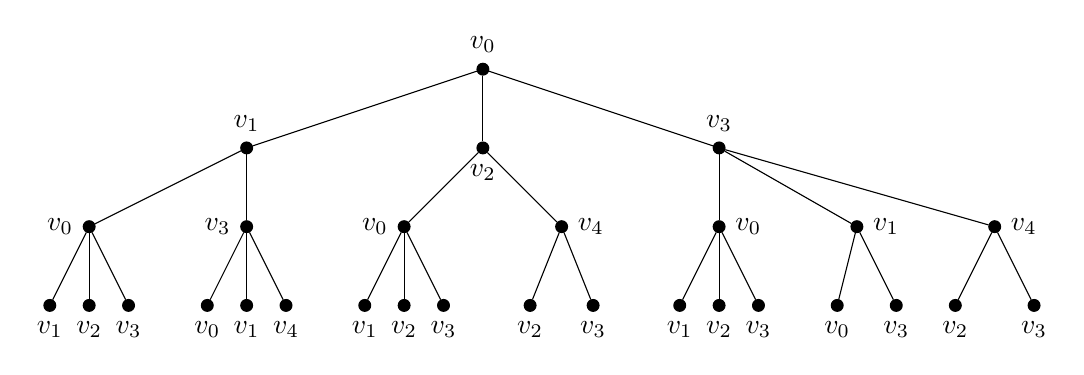
\begin{tikzpicture}

      \tikzset{enclosed/.style={draw, circle, inner sep=0pt, minimum size=.15cm, fill=black}}
%% Vertices
      	\node[enclosed, label={above: $v_0$}] (v0) at (3,6) {};
      	\node[enclosed, label={above: $v_1$}] (v1) at (0,5) {};
    		\node[enclosed, label={below: $v_2$}] (v2) at (3,5) {};
  	    \node[enclosed, label={above: $v_3$}] (v3) at (6,5) {};
     	\node[enclosed, label={left: $v_0$}] (v4) at (-2,4) {};
     	\node[enclosed, label={left: $v_3$}] (v5) at (0,4) {};
     	\node[enclosed, label={left: $v_0$}] (v6) at (2,4) {};
     	\node[enclosed, label={right: $v_4$}] (v7) at (4,4) {};
     	\node[enclosed, label={right: $v_0$}] (v8) at (6,4) {};
     	\node[enclosed, label={right: $v_1$}] (v9) at (7.75,4) {};
     	\node[enclosed, label={right: $v_4$}] (v10) at (9.5,4) {};
     	\node[enclosed, label={below: $v_1$}] (v11) at (-2.5,3) {};
      	\node[enclosed, label={below: $v_2$}] (v12) at (-2,3) {};
  	    \node[enclosed, label={below: $v_3$}] (v13) at (-1.5,3) {};
  	    \node[enclosed, label={below: $v_0$}] (v14) at (-0.5,3) {};
     	\node[enclosed, label={below: $v_1$}] (v15) at (0,3) {};
     	\node[enclosed, label={below: $v_4$}] (v16) at (0.5,3) {};
     	\node[enclosed, label={below: $v_1$}] (v17) at (1.5,3) {};
      	\node[enclosed, label={below: $v_2$}] (v18) at (2,3) {};
  	    \node[enclosed, label={below: $v_3$}] (v19) at (2.5,3) {};
  	    \node[enclosed, label={below: $v_2$}] (v20) at (3.6,3) {};
  	    \node[enclosed, label={below: $v_3$}] (v21) at (4.4,3) {};
  	    \node[enclosed, label={below: $v_1$}] (v22) at (5.5,3) {};
      	\node[enclosed, label={below: $v_2$}] (v23) at (6,3) {};
  	    \node[enclosed, label={below: $v_3$}] (v24) at (6.5,3) {};
  	    \node[enclosed, label={below: $v_0$}] (v25) at (7.5,3) {};
     	\node[enclosed, label={below: $v_3$}] (v26) at (8.25,3) {};
     	\node[enclosed, label={below: $v_2$}] (v27) at (9,3) {};
     	\node[enclosed, label={below: $v_3$}] (v28) at (10,3) {};
%Edges
		\path (v0) edge node[midway, sloped, above] {} (v1);
		\path (v0) edge node[midway, sloped, above] {} (v2);
		\path (v0) edge node[midway, above] {} (v3);
		\path (v1) edge node[near end, sloped, below] {} (v4);
		\path (v1) edge node[midway, below] {} (v5);
		\path (v2) edge node[near end, sloped, above] {} (v6);
		\path (v2) edge node[near end, sloped, above] {} (v7);
		\path (v3) edge node[near end, sloped, above] {} (v8);
		\path (v3) edge node[near end, sloped, above] {} (v9);
		\path (v3) edge node[near end, sloped, above] {} (v10);
		\path (v4) edge node[near end, sloped, above] {} (v11);
		\path (v4) edge node[near end, sloped, above] {} (v12);
		\path (v4) edge node[near end, sloped, above] {} (v13);
		\path (v5) edge node[near end, sloped, above] {} (v14);
		\path (v5) edge node[near end, sloped, above] {} (v15);
		\path (v5) edge node[near end, sloped, above] {} (v16);
		\path (v6) edge node[near end, sloped, above] {} (v17);
		\path (v6) edge node[near end, sloped, above] {} (v18);
		\path (v6) edge node[near end, sloped, above] {} (v19);
		\path (v7) edge node[near end, sloped, above] {} (v20);
		\path (v7) edge node[near end, sloped, above] {} (v21);
		\path (v8) edge node[near end, sloped, above] {} (v22);
		\path (v8) edge node[near end, sloped, above] {} (v23);
		\path (v8) edge node[near end, sloped, above] {} (v24);
		\path (v9) edge node[near end, sloped, above] {} (v25);
		\path (v9) edge node[near end, sloped, above] {} (v26);
		\path (v10) edge node[near end, sloped, above] {} (v27);
		\path (v10) edge node[near end, sloped, above] {} (v28);

	\end{tikzpicture}
	\caption{De mulige løsninger for veje med længde 3 fra $v_{0}$ til $v_{k}$}
	\label{fig.vaegtetopg}
\end{figure}

Antallet af veje fra $v_{0}$ til $v_{2}$ er 5 og antallet af veje fra $v_{0}$ til $v_{3}$ er 6. Vi kan derfor opstille
\textbf{$A^{4}$}$=b_{1i} \cdot a_{1j}+b_{2i} \cdot a_{2j}=5 \cdot 1+6 \cdot 1=11$
Her er $b_{1i}$ antallet af veje fra $v_{i}=v_{0}$ til vores første $v_{k}=v_{2}$ og $a_{1j}$ er antallet af kanter fra vores første $v_{k}=v_{2}$ til vores $v_{j}=v_{4}$. På samme måde optræder $b_{2i}$ og $a_{2j}$ for vores andet $v_{k}=v_{3}$. Der er altså 11 veje med længden 4 fra knuden $v_{0}$ til knuden $v_{4}$.

\end{exmp}

\subsection{Vægtede grafer}
En \emph{vægtet graf} er en graf, hvori kanterne eller knuderne får tildelt en numerisk værdi. I dette projekt arbejdes der udelukkende med vægtede kanter, og vi vil derfor kun fokusere på dem i dette afsnit.
En vægtet graf er defineret ved:
\begin{defn}[Vægtede grafer]
En vægtet graf, $G=(V,E,w)$, består af en mængde knuder, $V$, en mængde kanter, $E$, og \emph{vægtfunktionen}, $w: E \rightarrow \R$.
\end{defn}

For en vægtet graf har alle kanter $e\in E$ en numerisk vægt, givet ved funktionen $w (e)$. Da $e$ er en kant incident med $\{u,v\}$ kan man ligeledes skrive $w (u,v)$. På samme måde som med uvægtede grafer, kan en vægtet graf også opdeles i de seks graftyper fundet i tabel \ref{tab:typer}.
\begin{figure}[H]
\centering
	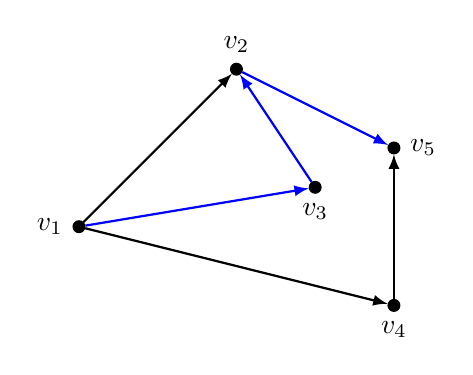
\begin{tikzpicture}

      \tikzset{enclosed/.style={draw, circle, inner sep=0pt, minimum size=.15cm, fill=black}}
%% Vertices
      	\node[enclosed, label={left: $v_1$}] (v1) at (0,2) {};
      	\node[enclosed, label={below: $v_3$}] (v2) at (3,2.5) {};
    		\node[enclosed, label={below: $v_4$}] (v3) at (4,1) {};
  	    \node[enclosed, label={above: $v_2$}] (v4) at (2,4) {};
     	\node[enclosed, label={right: $v_5$}] (v5) at (4,3) {};
%Edges
		\path [->, >=latex, thick, blue](v1) edge node[midway, sloped, above] {} (v2);
		\path [->, >=latex, thick](v1) edge node[midway, sloped, above] {} (v3);
		\path [->, >=latex, thick](v1) edge node[midway, above] {} (v4);
		\path [->, >=latex, thick, blue](v2) edge node[near end, sloped, below] {} (v4);
		\path [->, >=latex, thick](v3) edge node[midway, below] {} (v5);
		\path [->, >=latex, thick, blue](v4) edge node[near end, sloped, above] {} (v5);

	\end{tikzpicture}
	\caption{Eksempel på en orienteret simpel graf og en vej fra $v_{1}$ til $v_{5}$}
	\label{fig.vaegtetopg}
\end{figure}

Da vægtede grafer har en numerisk vægt på hver kant, kan man således beregne \emph{distancen} fra en knude til en anden i grafen. Distancen fra en knude til en anden kan defineres således:

\begin{defn}[Distance]
Lad $m\in \N $, $G=(V,E,w)$ være en vilkårlig graf og  $e_{v_i,v_{i+1}}$ være en kant, som er incident med $v_i$ og $v_{i+1}$. Lad en tilfældig, simpel vej, $P$, gå igennem knuderne således $P=(v_{1},v_{2},\dotsc,v_{m})$, da kan distancen beskrives som
	\begin{equation*}
	\mathrm{dist}(P)=\sum_{i=1}^{m}w(e_{v_i,v_{i+1}}).
	\end{equation*}  
\end{defn}

Man kan således bruge følgende definitioner af \emph{korteste vej} og \emph{længste vej} i en vægtet graf:


\begin{defn} [Korteste vej i vægtet graf]\label{defn:min.vej}
Lad $G=(V,E,w)$ være en vilkårlig, vægtet graf. Da er distancen af den korteste vej, fra en knude, $v_1$, til en anden knude, $v_m$, defineret som
	\begin{equation*}
		\alpha(v_1,v_m)=\arg \min_{P \in \euscr{P}}
		\textrm{dist}(P),
	\end{equation*}
	hvor $\euscr{P}$ er mængden af alle veje fra $v_1$ til $v_m$.
\end{defn}

På samme vis defineres længste vej:

\begin{defn} [Længste vej i en vægtet graf]
	Lad $G=(V,E,w)$ være en vilkårlig, vægtet graf. Da er distancen af den længste vej, fra en knude, $v_1$, til en anden knude, $v_m$, defineret som
	\begin{equation*}
		\beta(v_1,v_m)=\arg \max_{P \in \euscr{P}}
		\textrm{dist}(P),
	\end{equation*}
	hvor $\euscr{P}$ er mængden af alle veje fra $v_1$ til $v_m$.
\end{defn}

\begin{exmp}
Betragt figur \ref{fig.vaegtetopg} \\
\begin{figure}[H]
\centering
	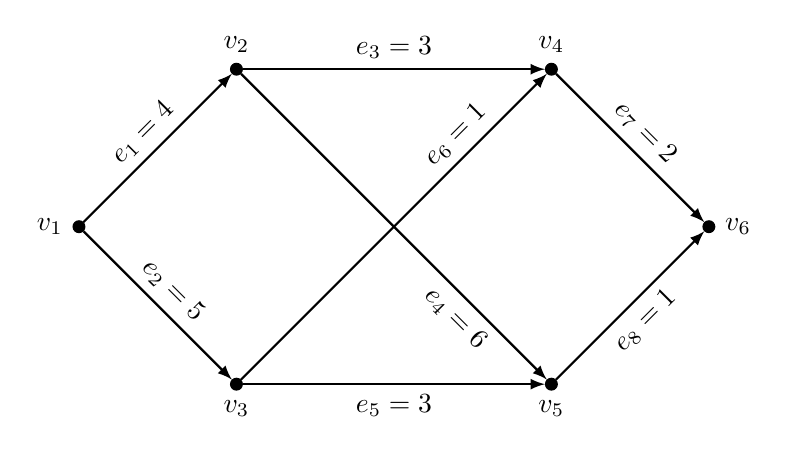
\begin{tikzpicture}

      \tikzset{enclosed/.style={draw, circle, inner sep=0pt, minimum size=.15cm, fill=black}}
%% Vertices
      	\node[enclosed, label={left: $v_1$}] (v1) at (0,2) {};
      	\node[enclosed, label={above: $v_2$}] (v2) at (2,4) {};
    	\node[enclosed, label={below: $v_3$}] (v3) at (2,0) {};
  	    \node[enclosed, label={above: $v_4$}] (v4) at (6,4) {};
     	\node[enclosed, label={below: $v_5$}] (v5) at (6,0) {};
     	\node[enclosed, label={right: $v_6$}] (v6) at (8,2) {};
%Edges
		\path [->, > = latex, thick] (v1) edge node[midway, sloped, above] {$e_1=4$} (v2);
		\path [->, > = latex, thick] (v1) edge node[midway, sloped, above] {$e_2=5$} (v3);
		\path [->, > = latex, thick] (v2) edge node[midway, above] {$e_3=3$} (v4);
		\path [->, > = latex, thick] (v2) edge node[near end, sloped, below] {$e_4=6$} (v5);
		\path [->, > = latex, thick] (v3) edge node[midway, below] {$e_5=3$} (v5);
		\path [->, > = latex, thick] (v3) edge node[near end, sloped, above] {$e_6=1$} (v4);
		\path [->, > = latex, thick] (v4) edge node[midway, sloped, above] {$e_7=2$} (v6);
		\path [->, > = latex, thick] (v5) edge node[midway, sloped, below] {$e_8=1$} (v6);

	\end{tikzpicture}
	\caption{En simpel, orienteret og vægtet graf.}
	\label{fig.vaegtetopg}
\end{figure}


På figuren ses en graf med vægtede kanter. Vi er interesserede i at finde den korteste vej fra $v_1$ til $v_6$. For at finde den korteste vej, kigger vi på alle de mulige veje fra $v_1$ til $v_6$.
Følgende veje ses:
\begin{align*}
	P_1=&(v_1,v_2,v_4,v_6)\\
	P_2=&(v_1,v_2,v_5,v_6)\\
	P_3=&(v_1,v_3,v_5,v_6)\\
	P_4=&(v_1,v_3,v_4,v_6)
\end{align*}
Man kan nu beregne distancen af de fire veje, ved at tage summen af de kanter, vejen følger. Man får derved:
\begin{align*}
	P_1=&4+3+2=9\\
	P_2=&4+6+1=11\\
	P_3=&5+3+1=9\\
	P_4=&5+1+2=8
\end{align*}
Det ses, at den korteste vej fra $v_1$ til $v_6$ er $P_4$. 
Det er sådan, man kan finde korteste vej i en vægtet graf. Denne metode kaldes \emph{brute force}. Metoden kan blive meget tidskrævende ved mere komplekse grafer. I disse tilfælde vil man bruge alternative, bedre algoritmer til at løse problemet. Dette vil vi komme ind på senere i kapitel \ref{kap.algo}.
\end{exmp}


\section{Delte grafer}
I visse tilfælde kan en graf deles op for at optimere en algoritme til løsningen af en given problemstilling.
To mulige grafopdelinger er delgrafer og $k$-delte grafer.

\begin{defn}[Delgraf] \label{defn:delgraf} %subgraph
En \emph{delgraf} af grafen, $G= (V,E)$, er en graf, $D = (W,F)$, skabt af delmængderne af kanterne, $F \subseteq E$, og knuderne, $W \subseteq V$, hvori det gælder $F \subseteq (\{u,v\} | u,v \in W)$.
\end{defn}

En delgraf er \emph{induceret}, hvis mængden af kanter, $F$, indeholder alle kanter fra $E$, hvis knuder indgår i $W$.
Delgrafen kaldes \emph{udspændende} hvis $W=V$. 

\begin{defn}[\emph{k}-delt] \label{defn:k-delt} %k-partite
En graf, $G = (V, E)$, kaldes en \emph{$k$-delt graf}, hvis $V$ kan deles op i $k$ ikke-tomme delmængder, $V_1, V_2,\dotsc, V_k$, således at $V= V_1 \bigcup V_2 \bigcup \dotsc \bigcup V_k$. Foruden gælder det at $V_i \bigcap V_j  = \emptyset \forall i,j$, og $i\neq j$. Samtidigt kan to vilkårlige knuder, $v$ og $u$, kun være naboer, hvis de befinder sig i forskellige delmængder. 
\end{defn}

Vi ved fra \autoref{kap:vaegtede}, at den optimale delstruktur findes, når man løser et korteste vej-problem. Dermed findes den optimale delstruktur, $D_{ij}$, hvis den optimale delgraf, $D$, er fundet.









